\documentclass[12pt]{article}
 
\usepackage[margin=1in]{geometry} 
\usepackage{amsmath,amsthm,amssymb}
\usepackage[spanish]{babel}
\usepackage{tikz}
\usepackage{tikz-cd}
\usetikzlibrary{babel}
\usepackage[utf8]{inputenc}
\usepackage{amsmath}
\usepackage[shortlabels]{enumitem}
\usepackage{mathtools}
\usepackage{xcolor}
\usepackage{float}
\usepackage{url}

\newtheorem{theorem}{Teorema}
\newtheorem{lemma}[theorem]{Lema}
\newtheorem{prop}[theorem]{Proposición}
\newtheorem{coro}[theorem]{Corolario}
\newtheorem{conj}[theorem]{Conjetura}
\newtheorem{ejercicio}{Ejercicio}
\newtheorem*{ejercicio*}{Ejercicio}
\theoremstyle{definition}
\newtheorem{definition}[theorem]{Definición}
\newtheorem{example}[theorem]{Ejemplo}
\theoremstyle{remark}
\newtheorem{remark}[theorem]{Nota}
\newtheorem{notacion}[theorem]{Notación}
 
\graphicspath{{img/}}
\decimalpoint

\begin{document}


\title{Apuntes}
\maketitle

\section{Conceptos básicos}

\begin{definition}
Un rayo es una función $P(t)=A+tb$, donde $P(t)$ es un punto 3D, $A$ es el origen del rayo y $b$ es la dirección del rayo.
\end{definition}

\begin{definition}
El \textit{viewport} es un rectángulo 2D usado para proyectar la escena 3D a la posición de la cámara virtual. En otras palabras, el viewport es una región de la pantalla usada para mostrar parte de la imagen total. 
\end{definition}

\begin{definition}
La \textit{focal length} es la distancia entre el plano de proyección y el punto de proyección. Esta distancia es distinta a la \textit{focus distance}.
\end{definition}

\begin{definition}
A \textit{linear blend}, interpolación lineal o \textit{lerp} es de la forma:
\[
\text{blendedValue} = (1-t)\cdot\text{startValue}+t\cdot\text{endValue}, \; t\in[0,1]
\]
\end{definition}

\begin{prop}
Sea $r$ la dirección de un rayo y $n$ la normal (hacia afuera) de una superficie intersecada por el rayo. Si $r\cdot n>0$, entonces el rayo se encuentra dentro de la superficie. En caso contrario, se encontrará fuera.
\end{prop}

\begin{proof}
Basta usar que $a\cdot b = |a||b|\cos\theta$ y la gráfica del coseno para ver su signo.
\end{proof}

\begin{definition}

El \textit{antialiasing} es un filtro que suaviza los \textit{dientes de sierra} que se crean al intentar pintar líneas curvas. 

\begin{figure}[H]
   \center
  
\includegraphics[scale=0.6]{antialiasing.png}
  \caption{Imagen tomada de \cite{antialiasing}}
\end{figure}

\end{definition}

\section{Convenciones}

\begin{enumerate}

\item Vamos a tomar el sistema de referencia siguiente para la cámara:

\begin{figure}[H]
   \center
  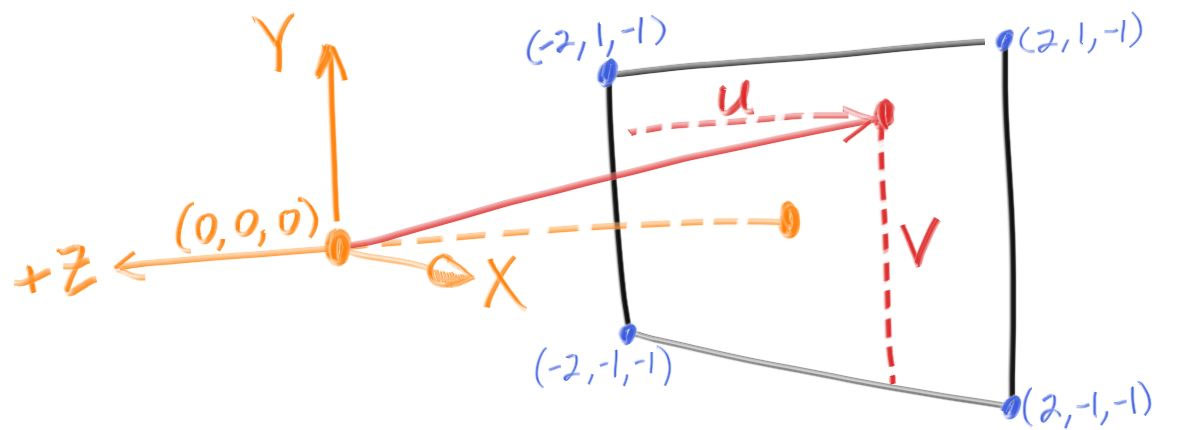
\includegraphics[scale=0.3]{camera_convention.jpg}
  \caption{Imagen tomada de \cite{first_book}}
\end{figure}

\item Las normales siempre apuntan hacia afuera de la superficie. Si en su lugar tomáramos las normales siempre apuntando contrarias al rayo, entonces no podríamos usar el producto vectorial para determinar en qué lado de la superficie estamos. Por tanto, sería necesario guardar esa información.

\end{enumerate}

\section{Materiales}

\subsection{Materiales difusos/mates}

Los objetos difusos o mates no emiten luz, simplemente toman el color del ambiente en el que se encuentran, alterandolo ligeramente con su propio color. La dirección de la luz reflejada por un material difuso es aleatoria.

\begin{figure}[H]
   \center
  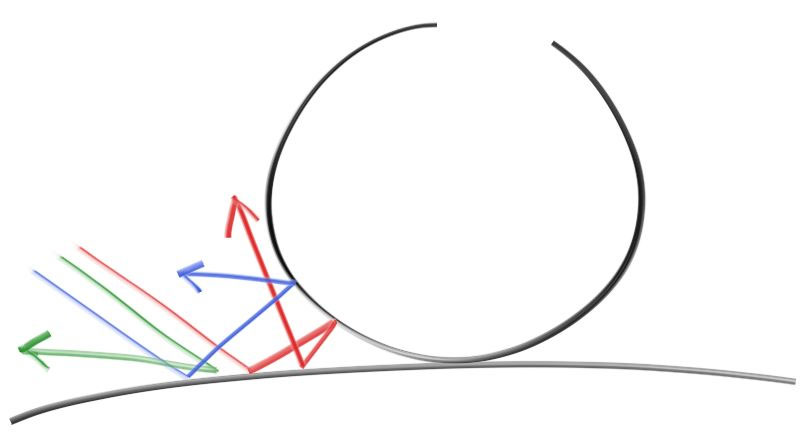
\includegraphics[scale=0.3]{diffuse.jpg}
  \caption{Imagen tomada de \cite{first_book}}
\end{figure}

\subsubsection{Elección de rayos}

Los rayos también podrían ser absorvidos en lugar de reflejados. Cuanto más oscura sea la superficie, más probable es que sea absorvido.

\begin{figure}[H]
   \center
  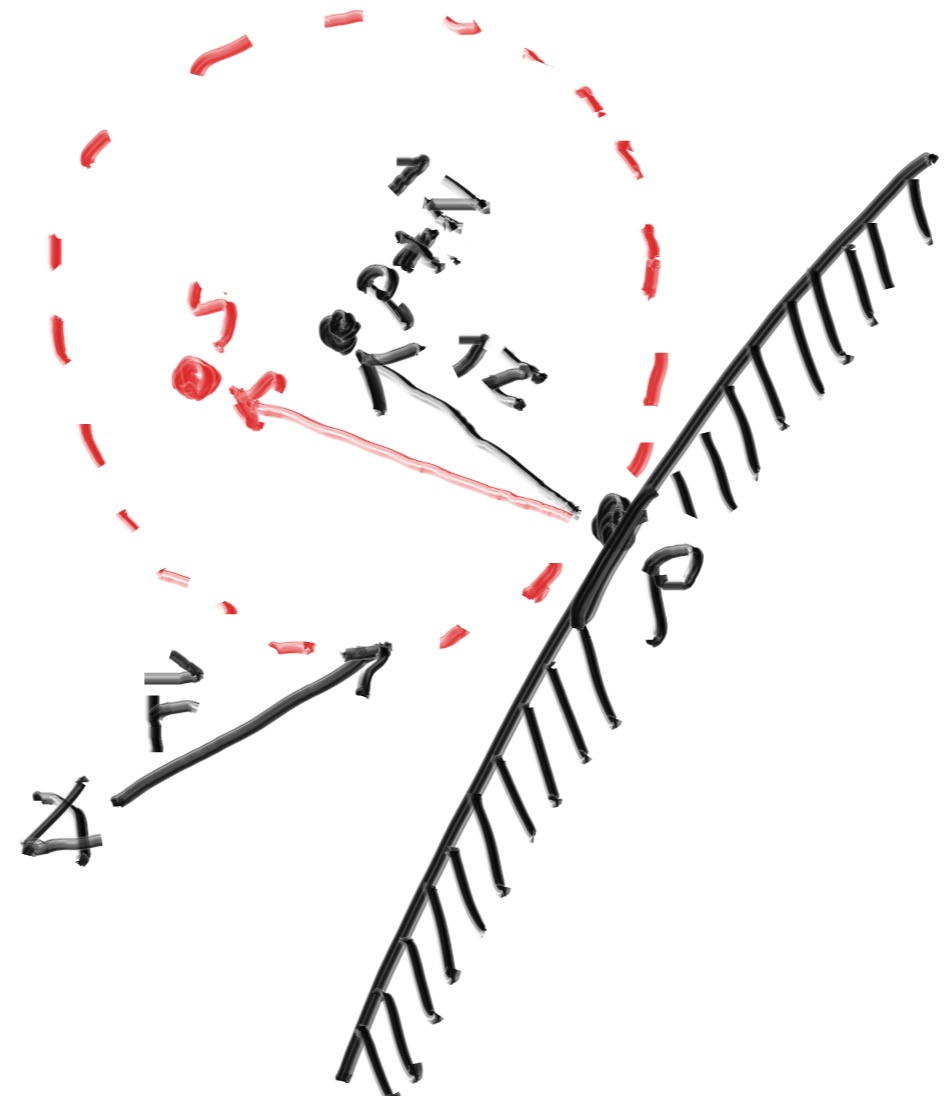
\includegraphics[scale=0.2]{diffuse_tangent.jpg}
  \caption{Imagen tomada de \cite{first_book}}
\end{figure}

El punto $S$ es eligido de forma aleatoria dentro de la esfere tangente a $P$ de radio unidad (la de centro $P+n$). El nuevo rayo reflejado será el que pasa por el punto $P$ con dirección $S-P$.

\subsubsection{Corrección gamma}

Es una operación no linear, usada para codificar y decodificar la luminosidad. Es definido por la siguiente fórmula:
\[
V_{out}=AV_{in}^\gamma
\]
Dependiendo del valor de $\gamma$, la luminosidad de la imagen variará:
\begin{itemize}
\item $\gamma < 1$: normalmente denotado por \textit{encoding gamma} o \textit{gamma compression}. Cuánto más pequeño sea $\gamma$, más clara será la imagen resultante.
\item $\gamma > 1$: normalmente denotado por \textit{decoding gamma} o \textit{gamma decompression}. Cuánto más grande sea $\gamma$, más oscura será la imagen resultante.
\end{itemize}

En nuestro programa, tomamos $A=\frac{1}{nsamples}$ donde $nsamples$ es el número de rayos creados por pixel, y $\gamma=\frac{1}{2}$.

\subsubsection{Shadow Acne}

Algunos de los rayos reflejados, debido a las aproximaciones usadas, intersecan el propio objeto que los está reflejando, luego hay que ignorar los valores de $t$ muy pequeños. Por ejemplo, sólo considerar intersecciones a partir de $t=0.001$.

\subsubsection{Reflexión Lambertiana}

Después de leer \cite{lambertian}, no me queda muy claro esto.

\subsection{Materiales metálicos}

En el caso de metales suaves el rayo no es dispersado aleatoriamente, sino que es reflejado con el mismo ángulo de incidencia pero al otro lado de la normal (ver \cite{beam}).

\begin{figure}[H]
\centering
\begin{tikzpicture}
  \draw[line width=1pt](-4,0)--(4,0);
  \draw[line width=1pt,blue,-stealth](0,0)--(2,2) node[anchor=south west]{$r$};
  \draw[line width=1pt,red,-stealth](-2,2)--(0,0) node[anchor=north east]{$v$};
  \draw [domain=45:135] plot ({0.5*cos(\x)}, {0.5*sin(\x)});
  \node[] at (0.25, 0.7) {$\theta$};
  \node[] at (-0.25, 0.7) {$\theta$};
  \draw[line width=1pt,red,-stealth](0,0)--(2,-2) node[anchor=north east]{$v$};
  \draw[line width=1pt,black,dashed,->](0,0)--(0,1.5) node[anchor=south]{$n$};
  \draw[line width=1pt,dashed,->](2,-2)--(2,0) node[anchor=north west]{$b$};
  \draw[line width=1pt,dashed,->](2,0)--(2,2) node[anchor=north west]{$b$};
  \draw[line width=1pt,dashed,|-|](0,0)--(0,-2);
  \node[] at (-0.8, -1) {$|v|\cos\theta$};
\end{tikzpicture}
\caption{Reflexión}
\end{figure}

A partir del dibujo se ve que la dirección del rayo reflejado es $r=v+2b$. El vector $b$ puede ser calculado usando $n$, que es unitario, y el hecho de que $v\cdot n=|v||n|\cos\theta=|v|\cos\theta$. Como $\angle (v,n)> \frac{\pi}{2}$, $dot(v,n)$ es negativo, luego es necesario añadir un signo menos, quedando:
\[
r=v-2dot(v,n)*n
\]

Una vez calculado el vector reflejado, es posible añadir un grado de \textit{fuzziness} al metal sumando un vector aleatorio a $r$. 

\begin{figure}[H]
\centering
\begin{tikzpicture}
  \draw[line width=1pt](-4,0)--(4,0);
  \draw[line width=1pt,blue,-stealth](0,0)--(2,2);
  \node[blue] at (1, 1.3) {$r$};
  \draw[line width=1pt,red,-stealth](-2,2)--(0,0);
  \node[red] at (-1, 1.3) {$v$};
  \draw[line width=1pt,green,-stealth](0,0)--(2.2,1.8);
  \node[green] at (1, 0.6) {$r'$};
  \draw[line width=1pt,dashed,-stealth](2,2)--(2.2,1.8);
  \node[scale=0.6] at (2.2, 2.05) {$p$};
  \draw[dashed] (2,2) circle (0.5);
\end{tikzpicture}
\end{figure}


donde $p\in B(0,1)$, es un vector aleatorio. Cuanto más grande sea el radio de la bola escogida, más borrosa se verá la imagen. Hay que ser precavido con la elección del radio, ya que si es demasiado grande, el rayo reflejado podría volver a intersecar nuestra superficie.

\subsection{Materiales dieléctricos}

Cuando un rayo alcanza un material dieléctrico (como agua, cristal, etc.), el rayo es dividido en dos partes: un rayo reflejado y otro refractado. La refracción es descrita por la \textit{ley de Snell}:
\[
\eta\sin\theta=\eta'\sin\theta'
\]
donde $\theta$ y $\theta'$ son los ángulos, medidos desde la normal, y $\eta$ y $\eta'$ son los coeficientes de reflexión de los medios, respectivamente.

\begin{figure}[H]
\centering
\begin{tikzpicture}
  \draw[line width=1pt](-2.5,0)--(2.5,0);
  \draw[line width=1pt, dashed](0,-2.5)--(0,2.5);
  \draw[line width=1pt,blue,-stealth](-2,2)--(0,0);
  \draw[line width=1pt,blue,-stealth](0,0)--(1,-2);
  \draw [domain=90:135] plot ({0.5*cos(\x)}, {0.5*sin(\x)});
  \draw [domain=270:295] plot ({0.5*cos(\x)}, {0.5*sin(\x)});
  \node[] at (-2, 0.3) {$\eta$};
  \node[] at (-2, -0.3) {$\eta'$};
  \node[] at (-0.3, 0.6) {$\theta$};
  \node[] at (0.25, -0.8) {$\theta'$};
\end{tikzpicture}
\caption{Refracción}
\end{figure}

Para determinar la dirección del rayo refractado es necesario resolver la ley de Snell, averiguando el valor de $\sin\theta'$, es decir, hay que resolver $\sin\theta'=\frac{\eta}{\eta'}\sin\theta$.

\begin{figure}[H]
\centering
\begin{tikzpicture}
  \draw[line width=1pt](-2.5,0)--(2.5,0);
  \draw[line width=1pt, dashed](0,-2.5)--(0,2.5);
  \draw[line width=1pt,blue,-stealth](-2,2)--(0,0);
  \draw[line width=1pt,blue,-stealth](0,0)--(1,-2);
  \draw [domain=90:135] plot ({0.5*cos(\x)}, {0.5*sin(\x)});
  \draw [domain=270:295] plot ({0.5*cos(\x)}, {0.5*sin(\x)});
  \node[] at (-0.3, 0.6) {$\theta$};
  \node[] at (0.25, -0.8) {$\theta'$};
  \node[blue] at (-2, 1.7) {$R$};
  \node[blue] at (1, -2.3) {$R'$};
  \draw[line width=1pt,red,dashed,->](0,0)--(0,-2);
  \node[red,scale=0.8] at (-0.4, -1.2) {$R'_{||}$};
  \draw[line width=1pt,red,dashed,->](0,0)--(1,0);
  \node[red,scale=0.8] at (0.5, 0.3) {$R'_{\perp}$};
  \draw[line width=1pt,red,dashed](1,0)--(1,-2);
  \draw[line width=1pt,red,dashed](0,-2)--(1,-2);
  \draw[line width=1pt,->](0,0)--(0,0.8);
  \draw[line width=1pt,->](0,0)--(0,-0.8);
  \node[] at (0.3, 0.8) {$n$};
  \node[] at (-0.3, -0.6) {$n'$};
\end{tikzpicture}
\end{figure}

Sea $R'$ el rayo refractado y $R$ el rayo incidente. $n$ y $n'$ son las normales a cada lado de la superficie. $R'$ se puede expresar como la suma de dos vectores, uno perpendicular y otro paralelo a $n'$: $R'=R'_{\perp}+R'_{||}$. Ahora hay que determinar esos dos vectores
\begin{itemize}
\item Usando que $\sin\theta=R+\cos\theta n$, se tiene que $R'_{\perp}=\sin\theta'=\frac{\eta}{\eta'}\sin\theta=\frac{\eta}{\eta'}(R+\cos\theta n)$.
\item Asumiendo que $R'$ es unitario, se puede usar el teorema de Pitágoras para calcular el módulo de $R'_{||}$. Como fue asumido que las normales apuntarían hacia afuera, no se puede usar $n'$, sino que hay que usar $n$, pero $n'=-n$. Luego: $R'_{||}=-\sqrt{1-|R'_{\perp}|^2}n$.
\end{itemize}
Ahora queda resolver la ecuación para $\cos\theta$. Suponiendo que $R$ sea unitario, se tiene que $dot(R,n)=|R||n|\cos\theta=\cos\theta$. Como el ángulo entre $R$ y $n$ es superior a 90 grados, su producto escalar será negativo, luego es necesario poner un signo menos, quedando:
\[
\begin{array}{ll}
R'_{\perp}=\frac{\eta}{\eta'}(R+(-R\cdot n)n)\\
R'_{||}=-\sqrt{1-|R'_{\perp}|^2}n
\end{array}
\]

En el procedimiento anterior hay un problema: si el rayo pasa del material con mayor coeficiente de refracción al de menor, entonces no hay una solución real a la ley de Snell. Por ejemplo, suponiendo $\eta=1.5$ (cristal) y $\eta'=1.0$ (aire) se tendría:
\[
\sin\theta'=\frac{1.5}{1.0}\sin\theta=1.5\sin\theta
\]
luego se podría dar el caso de que $1.5\sin\theta>1$, pero $\sin\theta'$ no puede ser mayor que 1. En esta situación, el material dieléctrico no puede refractar rayos, solo reflejarlos. Esto suele ocurrir cuando el rayo se encuentra dentro un material sólido. Este fenómeno se suele llamar \textit{reflexión interna total}.

Para la reflexión usamos la aproximación de Schilick (ver \cite{schlickapproximation}):
\[
R(\theta)=R_0+(1-R_0)(1-cos\theta)^5, \;\;\;\; R_0=\left(\frac{n_1-n_2}{n_1+n_2}\right)^2
\]
siendo $n1$ y $n2$ los coeficientes de refracción de cada medio.

\begin{thebibliography}{9}
\bibitem{first_book}
\url{https://raytracing.github.io/books/RayTracingInOneWeekend.html}
\bibitem{antialiasing}
\url{https://hardzone.es/reportajes/que-es/anti-aliasing-juegos/}
\bibitem{gamma_correction}
\url{https://en.wikipedia.org/wiki/Gamma_correction}
\bibitem{lambertian}
\url{https://en.wikipedia.org/wiki/Lambertian_reflectance}
\bibitem{beam}
\url{https://www.optics4kids.org/what-is-optics/reflection/the-reflection-of-light#:~:text=Polished%20metal%20surfaces%20reflect%20light,the%20metal%20surface%20is%20reflected.&text=The%20law%20of%20reflection%20requires,imaginary%20line%20(dashed%20in%20Fig.}
\bibitem{tikzmanual}
\url{https://www.bu.edu/math/files/2013/08/tikzpgfmanual.pdf}
\bibitem{snellslaw}
\url{https://en.wikipedia.org/wiki/Snell%27s_law}
\bibitem{schlickapproximation}
\url{https://en.wikipedia.org/wiki/Schlick%27s_approximation}
\end{thebibliography}

\end{document}